\documentclass[aspectratio=169]{beamer}

\usetheme{Madrid}
\usecolortheme{default}

\usepackage[utf8]{inputenc}
\usepackage[T1]{fontenc}
\usepackage[english]{babel}
\usepackage{amsmath}
\usepackage{listings}
\usepackage{xcolor}
\usepackage{booktabs}
\usepackage{graphicx}
\usepackage{tikz}
\usepackage{hyperref}

\lstset{
  basicstyle=\ttfamily\small,
  keywordstyle=\color{blue},
  commentstyle=\color{gray},
  stringstyle=\color{orange},
  breaklines=true,
  frame=single,
}

% ── Metadata ──────────────────────────────────────────────────────────────────
\title[Automated Data Collection]{Everything, Everywhere, All at Once}
\subtitle{Keynote on Automated Data Collection}
\author{Stephan Bökelmann}
\institute{PDSC4k – Practical Data Science Conference}
\date{2026}

% ── Document ──────────────────────────────────────────────────────────────────
\begin{document}

% Title slide
\begin{frame}
  \titlepage
\end{frame}

% ── Overview diagram ──────────────────────────────────────────────────────────
\begin{frame}{The Full Journey at a Glance}
  \begin{center}
    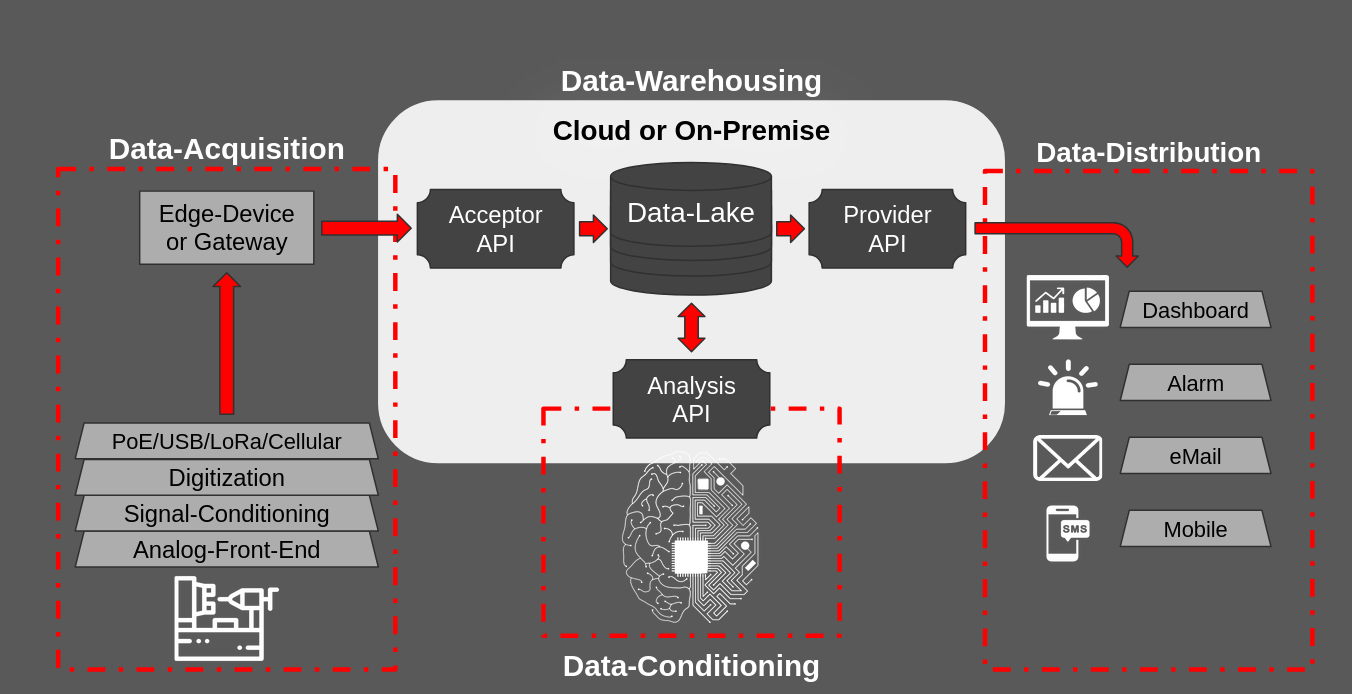
\includegraphics[width=0.92\textwidth]{architecture.png}
  \end{center}
  \vspace{-0.5em}
  \begin{center}
    \small Four zones — one owner per box.\\
    We will walk through them one by one.
  \end{center}
\end{frame}

% Table of contents
\begin{frame}{Agenda}
  \tableofcontents
\end{frame}

% ══════════════════════════════════════════════════════════════════════════════
\section{Data Acquisition}
% ══════════════════════════════════════════════════════════════════════════════

\begin{frame}{Data Acquisition: Where the Physical World Meets Software}
  \begin{columns}
    \column{0.55\textwidth}
      The stack from the bottom up:
      \begin{enumerate}
        \item \textbf{Analog Front-End} – amplification, filtering, impedance
        \item \textbf{Signal Conditioning} – offset, scaling, protection
        \item \textbf{Digitization} – ADC, sampling rate, resolution
        \item \textbf{Transport} – PoE / USB / LoRa / Cellular
        \item \textbf{Gateway} – passive network bridge (modem, LoRa base station)
        \item \textbf{Edge Compute} – first intelligent software node
      \end{enumerate}
    \column{0.4\textwidth}
      \begin{alertblock}{Garbage-in Problem}
        Errors in the lower layers are
        \textbf{not} fixable by later software.
        A miscalibrated sensor delivers
        plausible but wrong data.
      \end{alertblock}
  \end{columns}
\end{frame}

\begin{frame}{Analog Front-End and Signal Conditioning}
  What actually happens here — and why data scientists should care:
  \begin{itemize}
    \item \textbf{Aliasing}: Sampling rate must be $\geq 2\times$ the
          highest signal frequency (Nyquist)
    \item \textbf{Quantisation noise}: 12-bit ADC $\Rightarrow$
          $\approx 0.024\,\%$ resolution — is that enough?
    \item \textbf{Offset drift}: Temperature-dependent shift of the
          zero point $\Rightarrow$ systematic error
    \item \textbf{Electromagnetic interference}: Differential measurement,
          shielding, twisted pair
  \end{itemize}
  \vspace{0.5em}
  \begin{exampleblock}{Takeaway}
    Talk to the hardware engineers before you train your model.
  \end{exampleblock}
\end{frame}

\begin{frame}{Edge Compute: Gateway and Compute Node in One}
  \begin{columns}
    \column{0.42\textwidth}
      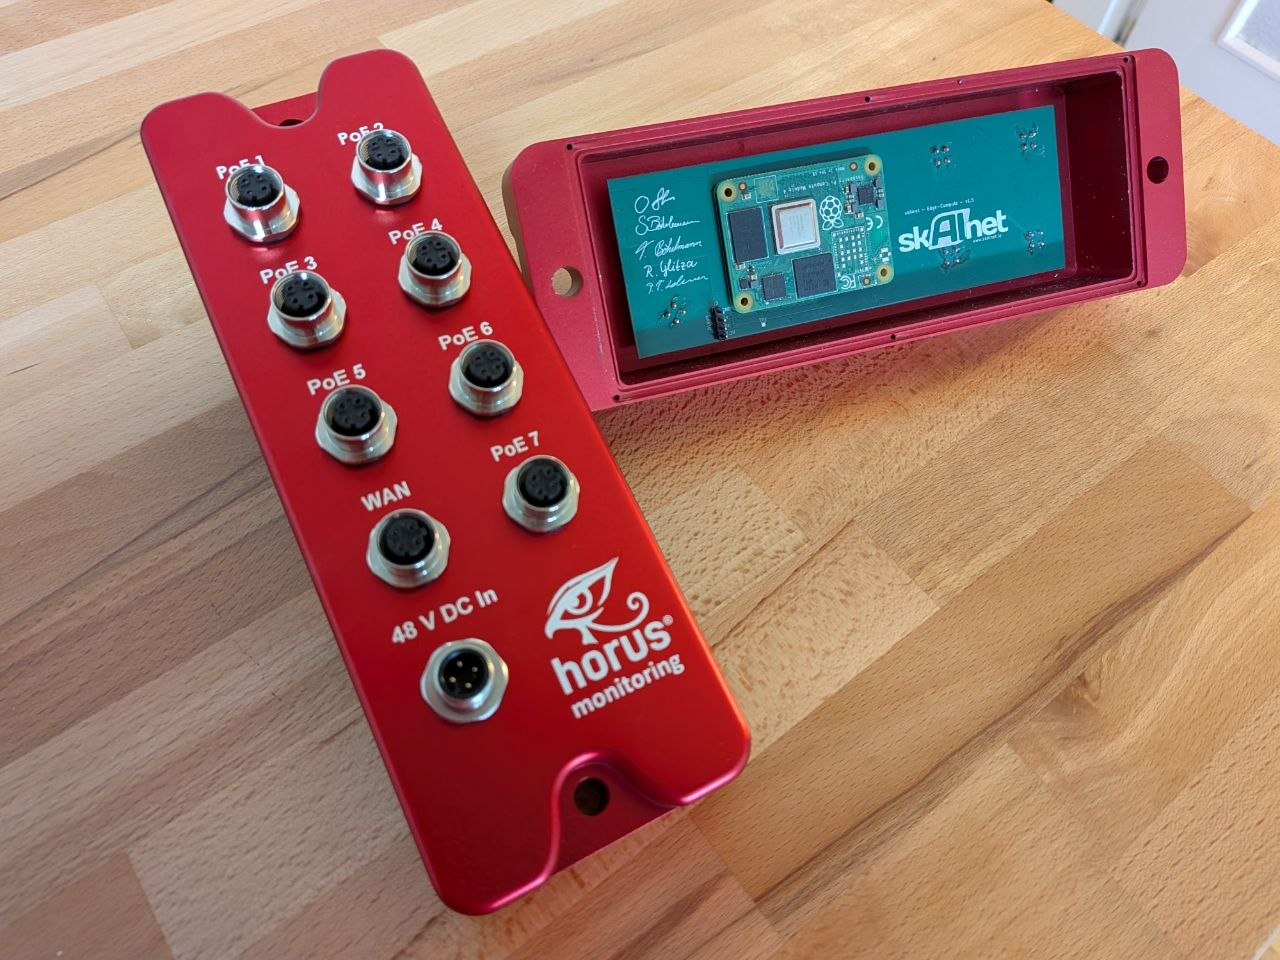
\includegraphics[width=\textwidth]{horus.png}
    \column{0.54\textwidth}
      \textbf{Horus Edge Compute Platform} (custom mainboard, SBC-agnostic):
      \begin{itemize}
        \item Integrated router with \textbf{two separate ETH interfaces}
              (WAN / LAN isolation)
        \item \textbf{7 PoE LAN ports} – sensors are powered directly
        \item \textbf{48\,V DC} supply, industrial grade
        \item Sensor discovery via \texttt{slook}
              (github: dominicpoeschko) through the Peripheral Access Daemon
        \item Calibration \& cleaning \textbf{locally}, before data
              travels over WAN to the Acceptor API
        \item Currently in development: variant with \textbf{NVIDIA Jetson} module
              for inference directly at the edge
      \end{itemize}
  \end{columns}
\end{frame}

\begin{frame}{Why Compute Belongs at the Edge}
  \begin{block}{Our Architectural Pattern}
    Sensors $\xrightarrow{\text{PoE/LAN}}$ Edge Compute
    $\xrightarrow{\text{WAN}}$ Acceptor API
  \end{block}
  \vspace{0.5em}
  What the Edge Compute does \textbf{before} the WAN:
  \begin{enumerate}
    \item \textbf{Aggregation} – bundle data from any number of channels
          (7 PoE ports, behind them any number of switches)
    \item \textbf{Calibration} – apply device-specific correction factors
    \item \textbf{Cleaning} – outliers, gaps, encoding errors
    \item \textbf{Buffering} – store-and-forward on WAN failure
  \end{enumerate}
  \vspace{0.5em}
  \begin{alertblock}{Rule of Thumb}
    Anything that can be \textbf{decided before} the WAN belongs at the edge –
    bandwidth is expensive, compute time at the edge is free.
  \end{alertblock}
\end{frame}

\begin{frame}{Transport Protocols Compared}
  \begin{columns}
    \column{0.48\textwidth}
      \begin{block}{Wired}
        \begin{itemize}
          \item \textbf{PoE}: power + data, simple, reliable
          \item \textbf{USB}: short distance, plug-and-play
          \item \textbf{Modbus RTU}: industrial standard, robust
        \end{itemize}
      \end{block}
    \column{0.48\textwidth}
      \begin{block}{Wireless}
        \begin{itemize}
          \item \textbf{LoRa}: long range, low bandwidth
          \item \textbf{Cellular (LTE-M)}: everywhere, but costly
          \item \textbf{BLE}: short range, battery-friendly
        \end{itemize}
      \end{block}
  \end{columns}
  \vspace{0.5em}
  \begin{alertblock}{The Forgotten Question}
    What happens to the data when the WAN connection is down for 3 hours?
    Store-and-forward on the \textbf{Edge Compute} is not optional –
    a passive gateway buffers nothing.
  \end{alertblock}
\end{frame}

\begin{frame}{Starlink: Satellite Internet as a WAN Option}
  \begin{columns}
    \column{0.55\textwidth}
      Starlink addresses the last blind spot in connectivity — \textbf{sites without infrastructure}:
      \begin{itemize}
        \item Latency currently $\approx 20$–$60\,\text{ms}$ (Low-Earth-Orbit)
        \item Bandwidth $\approx 50$–$200\,\text{Mbit/s}$ down
        \item \textbf{Starlink for IoT}: flat API programme for
              machine-to-machine communication, optimised for
              continuous operation with small packets
        \item Failover option alongside LTE-M for critical sites
        \item Hardware: compact flat-panel dish, weatherproof
      \end{itemize}
    \column{0.4\textwidth}
      \begin{block}{When Relevant?}
        \begin{itemize}
          \item Mines, offshore, construction sites
          \item Large-scale agriculture
          \item Temporary measurement campaigns
          \item Backup when cellular fails
        \end{itemize}
      \end{block}
      \begin{alertblock}{Caution}
        Data protection: check Starlink server locations (GDPR).
      \end{alertblock}
  \end{columns}
\end{frame}

% ══════════════════════════════════════════════════════════════════════════════
\section{Data Warehousing}
% ══════════════════════════════════════════════════════════════════════════════

\begin{frame}{Data Warehousing: Acceptor API $\rightarrow$ Data Lake}
  \begin{columns}
    \column{0.55\textwidth}
      The Acceptor API is the first software gate:
      \begin{itemize}
        \item Authentication and authorisation
        \item Schema validation (mandatory fields, types)
        \item Rate limiting against flooding
        \item Idempotency keys enforced
        \item Writing into the Data Lake (append-only)
      \end{itemize}
    \column{0.4\textwidth}
      \begin{exampleblock}{Design Principle}
        The Acceptor API \textbf{rejects or accepts} –
        it does not transform.
        Transformation belongs in Data Conditioning.
      \end{exampleblock}
  \end{columns}
\end{frame}

\begin{frame}{What Actually Belongs in the Lake?}
  \begin{columns}
    \column{0.48\textwidth}
      \begin{block}{Should Go In}
        \begin{itemize}
          \item \textbf{Calibrated measurements} – pre-processed at the edge
          \item \textbf{Device metadata} – ID, firmware, calibration state
          \item \textbf{Heartbeats} – proof that a device is silent
        \end{itemize}
      \end{block}
    \column{0.48\textwidth}
      \begin{alertblock}{Should \textbf{Not} Go In}
        \begin{itemize}
          \item Polling artefacts without a measurement value
          \item Duplicates from retries (filter, do not store)
          \item Internal diagnostic data from the Edge Compute
        \end{itemize}
      \end{alertblock}
  \end{columns}
  \vspace{0.5em}
  \begin{exampleblock}{Rule of Thumb}
    Everything required to reconstruct the state of the world
    \textbf{at the exact moment of measurement} – nothing more, nothing less.
  \end{exampleblock}
\end{frame}

\begin{frame}{Practice: Ceph as a Real Cloud Solution – with THGA}
  \begin{columns}
    \column{0.48\textwidth}
      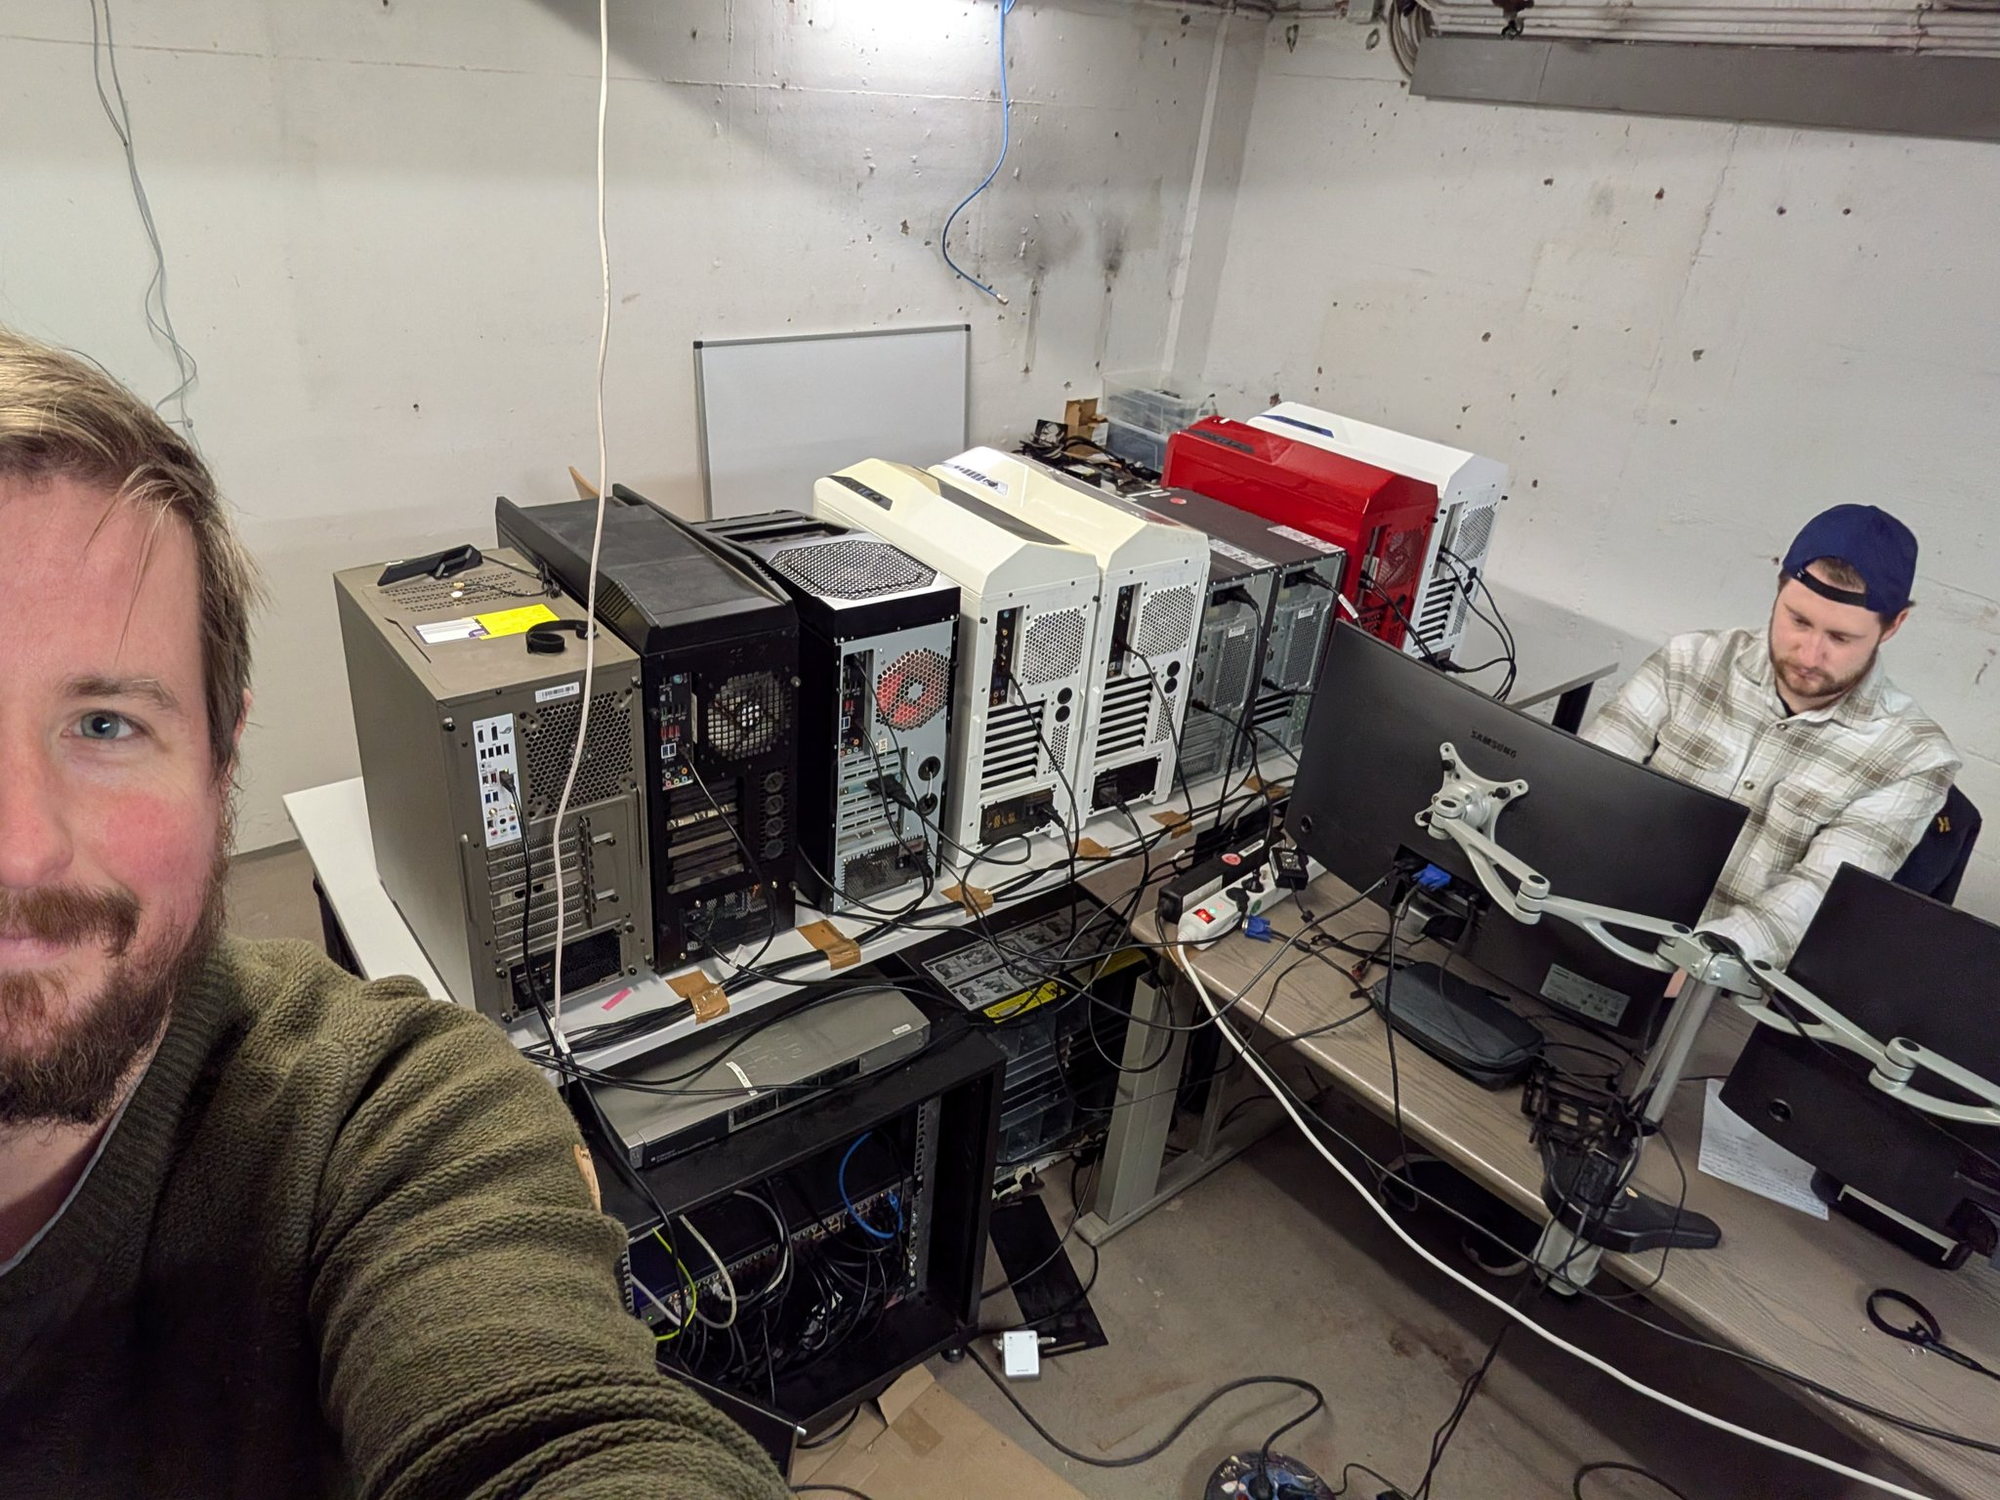
\includegraphics[width=\textwidth]{ceph.png}
    \column{0.48\textwidth}
      Philipp Lehmann and I, together with the
      \textbf{Technische Hochschule Georg Agricola (THGA)},
      have built a complete Ceph-based cloud infrastructure –
      no longer a proof of concept, but \textbf{running in production}:
      \begin{itemize}
        \item Currently \textbf{100\,TB usable} – and growing
        \item Real failure cases produced and analysed
        \item Paper in preparation
      \end{itemize}
      \vspace{0.5em}
      \begin{exampleblock}{}
        Philipp is here today –
        talk to him, he can tell you more.
      \end{exampleblock}
  \end{columns}
\end{frame}

\begin{frame}{IPFS as Storage Backend Behind the Acceptor}
  \begin{columns}
    \column{0.55\textwidth}
      \textbf{Architecture:}
      \begin{enumerate}
        \item Acceptor writes data $\rightarrow$ \textbf{IPFS node}
        \item IPFS returns a \textbf{CID} (Content Identifier = hash)
        \item CID + metadata $\rightarrow$ \textbf{On-Premise Metadata DB}
        \item \textbf{FastAPI catalogue} returns only metadata \& CID
        \item Consumer fetches the data themselves by CID from IPFS
      \end{enumerate}
    \column{0.4\textwidth}
      \begin{block}{Why IPFS?}
        \begin{itemize}
          \item CID is a checksum – no silent corruption
          \item Immutability by design
          \item Deduplication for free
          \item Storage location interchangeable (Ceph, S3, cluster)
        \end{itemize}
      \end{block}
      \begin{alertblock}{Separation}
        Metadata stays on-premise
        or in a separate cloud –
        never together with the data.
      \end{alertblock}
  \end{columns}
\end{frame}

\begin{frame}{Cloud vs. On-Premise: A Real Decision}
  \begin{columns}
    \column{0.48\textwidth}
      \begin{block}{Cloud}
        \begin{itemize}
          \item Elastic scaling
          \item No hardware operations
          \item Pay-per-use (watch out for egress costs!)
          \item GDPR: pay attention to server location
        \end{itemize}
      \end{block}
    \column{0.48\textwidth}
      \begin{block}{On-Premise}
        \begin{itemize}
          \item Data sovereignty
          \item Predictable fixed costs
          \item Air gap for critical systems
          \item Internal operational effort
        \end{itemize}
      \end{block}
  \end{columns}
  \vspace{0.5em}
  \begin{alertblock}{The Hybrid Reality}
    Acquisition on-premise, warehousing in the cloud – this is the most common
    compromise in industry.
  \end{alertblock}
\end{frame}

\begin{frame}{Backpressure: What Happens When Everyone Sends at Once?}
  \begin{alertblock}{The Scenario}
    50 Edge Computes send their buffered data simultaneously after a WAN outage –
    the Acceptor API gets flooded.
  \end{alertblock}
  \vspace{0.5em}
  \begin{columns}
    \column{0.32\textwidth}
      \textbf{Throttling (Acceptor):}
      \begin{itemize}
        \item \textbf{Token Bucket} – throughput per client
        \item \textbf{Circuit Breaker} – \texttt{503} on overload
        \item \textbf{Sliding Window} – bursts OK, sustained fire not
      \end{itemize}
    \column{0.32\textwidth}
      \textbf{Scaling (Infrastructure):}
      \begin{itemize}
        \item \textbf{k8s HPA} – new Acceptor pods under load
        \item \textbf{Load Balancer} – distributes across pod pool
        \item Design stateless – every pod is equal
      \end{itemize}
    \column{0.32\textwidth}
      \textbf{Buffering (Edge Compute):}
      \begin{itemize}
        \item \texttt{503} $\Rightarrow$ backoff + jitter
        \item Local buffer waits
        \item Fresh data first
      \end{itemize}
  \end{columns}
  \vspace{0.5em}
  \begin{exampleblock}{Core Idea}
    Throttling and scaling are not mutually exclusive –
    together they produce a robust system.
  \end{exampleblock}
\end{frame}

% ══════════════════════════════════════════════════════════════════════════════
\section{Data Conditioning}
% ══════════════════════════════════════════════════════════════════════════════

\begin{frame}{Data Conditioning: Where Data Learns to Think}
  \begin{center}
    The bidirectional connection in the diagram is not an accident:
  \end{center}
  \vspace{0.5em}
  \begin{columns}
    \column{0.48\textwidth}
      \textbf{Lake $\rightarrow$ Analysis API}
      \begin{itemize}
        \item Read raw data
        \item Clean, normalise
        \item Feature engineering
        \item Model inference
      \end{itemize}
    \column{0.48\textwidth}
      \textbf{Analysis API $\rightarrow$ Lake}
      \begin{itemize}
        \item Write derived features back
        \item Annotations, labels
        \item Model outputs as new datasets
        \item Aggregated views for distribution
      \end{itemize}
  \end{columns}
  \vspace{0.5em}
  \begin{exampleblock}{Key Idea}
    Conditioning \textbf{writes back} – the lake grows through analysis.
  \end{exampleblock}
\end{frame}

\begin{frame}{Analysis via a FastAPI Data Catalogue}
  \begin{columns}
    \column{0.55\textwidth}
      Instead of delivering data, the catalogue returns only \textbf{metadata}:
      \begin{itemize}
        \item Which datasets exist?
        \item CID / storage location in IPFS
        \item Time range, device, calibration state
        \item Quality status (validated / not validated)
      \end{itemize}
      \vspace{0.5em}
      The consumer decides what to load themselves –
      the catalogue never transports payload data.
    \column{0.4\textwidth}
      \begin{block}{Advantages}
        \begin{itemize}
          \item No central bottleneck
          \item Reproducibility: CID = exact data version
          \item Access control at the metadata level
          \item FastAPI: fast, type-safe, OpenAPI for free
        \end{itemize}
      \end{block}
      \begin{exampleblock}{}
        \texttt{GET /datasets?device=T42\&from=2026-01-01}\\
        \texttt{ \{cid, location, quality\}}
      \end{exampleblock}
  \end{columns}
\end{frame}

\begin{frame}{Orchestrating the Conditioning Pipelines}
  The orchestrator runs on the \textbf{analysis machine} –
  not in the warehouse. It queries the FastAPI catalogue for CIDs,
  loads data from IPFS, and writes results back.
  \vspace{0.3em}

  What orchestrators provide:
  \begin{itemize}
    \item Cron-like scheduling with dependency graphs (DAGs)
    \item Automatic retry with configurable policies
    \item Backfill: re-process missing time slices later
    \item Alerting on failure, SLA violation
    \item Audit log for every pipeline run
  \end{itemize}
  \vspace{0.5em}
  \begin{tabular}{ll}
    \toprule
    \textbf{Tool} & \textbf{Strength} \\
    \midrule
    Apache Airflow & Mature, large community, complex \\
    Prefect        & Python-native, easy to start \\
    dbt            & SQL-focused, transformation layer \\
    \bottomrule
  \end{tabular}
\end{frame}

% ══════════════════════════════════════════════════════════════════════════════
\section{Data Distribution}
% ══════════════════════════════════════════════════════════════════════════════

\begin{frame}{Data Distribution: Who Gets What, When, How?}
  \begin{columns}
    \column{0.55\textwidth}
      The Provider API is the \textbf{contractual boundary}
      to the outside world:
      \begin{itemize}
        \item Versioning (v1, v2 – never breaking)
        \item \textbf{Keycloak} – OIDC / OAuth2, role-based, SSO-capable
        \item Rate limiting per consumer
        \item Documentation (OpenAPI / AsyncAPI)
      \end{itemize}
    \column{0.4\textwidth}
      \begin{block}{Four Consumer Types}
        \begin{itemize}
          \item Dashboard (Pull, low latency)
          \item Alarm (Push, real-time)
          \item Email (asynchronous, batched)
          \item Mobile (Push notification)
        \end{itemize}
      \end{block}
  \end{columns}
\end{frame}

\begin{frame}{Provider API: FastAPI or Crow/C++ – and What Does the SLA Cost?}
  \begin{columns}
    \column{0.48\textwidth}
      \textbf{Technology Choice by Load:}
      \begin{tabular}{lll}
        \toprule
        & \textbf{FastAPI} & \textbf{Crow (C++)} \\
        \midrule
        Setup     & hours  & days \\
        Latency   & $\sim$5\,ms & $<$1\,ms \\
        Throughput & $\sim$10k\,req/s & $>$100k\,req/s \\
        Operations & easy  & complex \\
        \bottomrule
      \end{tabular}
      \vspace{0.5em}
      Rule of thumb: below $\sim$20k\,req/s FastAPI is the right choice –
      above that, C++ becomes worthwhile.
    \column{0.48\textwidth}
      \textbf{What the SLA Actually Means:}
      \begin{itemize}
        \item \textbf{Availability}: e.g. 99.9\,\% = max. 8.7\,h downtime/year – who pays below that?
        \item \textbf{Latency}: p99 $<$ 200\,ms – not the average, but the worst-case percentile
        \item \textbf{Freshness}: data at most $X$ minutes old
      \end{itemize}
      \vspace{0.3em}
      \begin{block}{k8s as Leverage}
        HPA scales Provider pods under load –
        SLA targets are maintained through scaling,
        not through over-provisioning.
      \end{block}
  \end{columns}
\end{frame}

\begin{frame}{Latency and Format Requirements per Consumer}
  \begin{tabular}{lllll}
    \toprule
    \textbf{Consumer} & \textbf{Latency} & \textbf{Format} &
    \textbf{Mechanism} & \textbf{Priority} \\
    \midrule
    Dashboard  & $<1\,s$    & JSON / REST    & Polling / WebSocket & Medium \\
    Alarm      & $<100\,ms$ & Minimal        & Webhook / MQTT      & Critical \\
    Email      & Minutes    & HTML / Text    & Queue               & Low \\
    Mobile     & $<5\,s$    & FCM / APNs     & Push notification   & High \\
    \bottomrule
  \end{tabular}
  \vspace{0.5em}
  \begin{alertblock}{Important}
    A single API endpoint for all consumers is an anti-pattern.
    Latency requirements are too different.
  \end{alertblock}
\end{frame}

\begin{frame}{Alerting Done Right}
  Common mistakes in alarm systems:
  \begin{itemize}
    \item \textbf{Alert fatigue}: too many alarms $\Rightarrow$ all are ignored
    \item \textbf{No hysteresis}: threshold flapping produces alarm storms
    \item \textbf{Wrong recipient}: alarm goes to everyone, nobody feels responsible
    \item \textbf{No context}: alarm without value, trend, or action instruction
  \end{itemize}
  \vspace{0.5em}
  \begin{exampleblock}{A Good Alarm}
    ``Sensor T-42 has exceeded $85\,°C$ for 3 minutes (currently $91\,°C$,
    trend: rising). Responsible: On-Call Mechanic. Runbook: \texttt{/wiki/T42}''
  \end{exampleblock}
\end{frame}

\begin{frame}{Separation of Responsibilities: Alarm, Analysis, Warehouse}
  \begin{alertblock}{Anti-Pattern: Everything on One Machine}
    When warehouse, analysis, and alerting share the same infrastructure,
    an outage takes down all three at once – exactly when alarms matter most.
  \end{alertblock}
  \vspace{0.5em}
  \begin{columns}
    \column{0.48\textwidth}
      \textbf{Three Separate Systems:}
      \begin{itemize}
        \item \textbf{Warehouse} – Acceptor, Lake, Provider API
        \item \textbf{Analysis} – Conditioning, FastAPI catalogue,
              ML pipelines
        \item \textbf{Alarm Service} – independent machine,
              sends email / SMS / push independently
      \end{itemize}
    \column{0.48\textwidth}
      \begin{block}{Trade-off}
        Higher initial setup effort –\\
        but every component is individually\\
        maintainable, scalable, and replaceable.
      \end{block}
      \begin{exampleblock}{Meta-Monitoring}
        \textbf{Uptime Kuma} (or similar) monitors
        the warehouse from the outside –
        monitoring the monitoring.
        Who watches the watcher?
      \end{exampleblock}
  \end{columns}
\end{frame}

% ══════════════════════════════════════════════════════════════════════════════
\section{The Diagram as a Checklist}
% ══════════════════════════════════════════════════════════════════════════════

\begin{frame}{Every Box Is a Responsibility Boundary}
  \begin{center}
    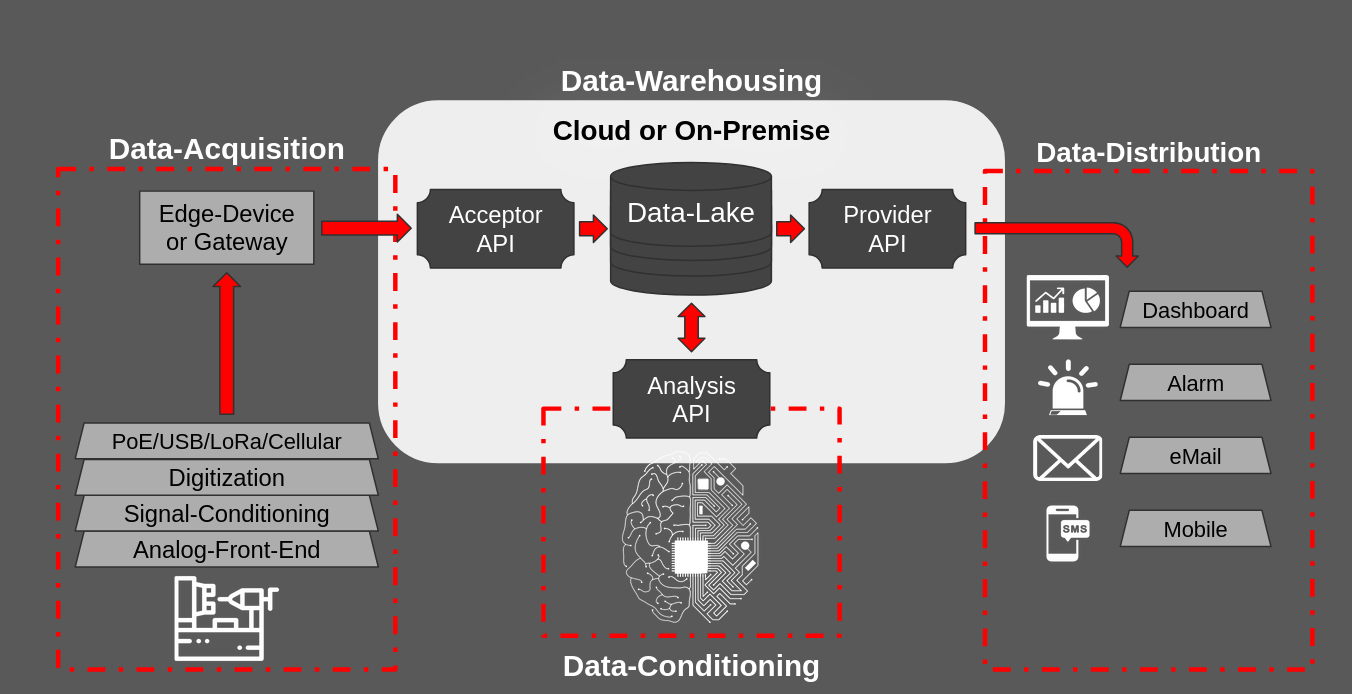
\includegraphics[width=0.82\textwidth]{architecture.png}
  \end{center}
  \vspace{-0.3em}
  \begin{center}
    \small Who \textbf{owns} which box in your organisation?
  \end{center}
\end{frame}

\begin{frame}{Checklist: Is Your Pipeline Production-Ready?}
  \begin{columns}
    \column{0.48\textwidth}
      \textbf{Data Acquisition}
      \begin{itemize}
        \item[$\square$] Calibration documented?
        \item[$\square$] Store-and-forward at the edge?
        \item[$\square$] Connection loss tested?
      \end{itemize}
      \textbf{Data Warehousing}
      \begin{itemize}
        \item[$\square$] Acceptor idempotent?
        \item[$\square$] Raw data stored immutably?
        \item[$\square$] \texttt{last\_write\_timestamp} monitored?
      \end{itemize}
    \column{0.48\textwidth}
      \textbf{Data Conditioning}
      \begin{itemize}
        \item[$\square$] Quality gates before every transformation?
        \item[$\square$] Backfill strategy documented?
        \item[$\square$] Derived data versioned?
      \end{itemize}
      \textbf{Data Distribution}
      \begin{itemize}
        \item[$\square$] Provider API versioned?
        \item[$\square$] Alarm hysteresis configured?
        \item[$\square$] Consumer latency tested?
      \end{itemize}
  \end{columns}
\end{frame}

\begin{frame}{Conclusion: Three Sentences to Take Away}
  \begin{enumerate}
    \item \textbf{Collecting data is engineering} –
          not a script that runs somewhere and hopes.
    \item \textbf{Quality is created at the source} –
          whatever the analog front-end corrupts, no model will save.
    \item \textbf{Every box needs an owner} –
          the largest data pipelines fail on unclear responsibility,
          not on technology.
  \end{enumerate}
\end{frame}

% ── Closing slide ─────────────────────────────────────────────────────────────
\begin{frame}
  \begin{center}
    {\Huge \textbf{Your turn.}}\\[1em]
    {\large Build pipelines that don't lie.}\\
    {\large Enjoy PDSC4k – and have a good exchange!}\\[2em]
    \textbf{Stephan Bökelmann}\\
    \texttt{stephan.boekelmann@gruppe.ai}\\[1em]
    \small
    \texttt{github.com/maxclerkwell/pdsc4k-talk}\\[0.4em]
    Collaboration: \texttt{www.skAInet.io}\\
    Blog: \texttt{maxclerkwell.github.io}
  \end{center}
\end{frame}

\end{document}